\section{VAE (Variational Autoencoder)}

I VAE permettono di costruire un \textbf{latent space continuo}; Permette di
prendere uno spazio e un sample da quello spazio e saremo certi che i punti
all'interno seguono la distribuzione di quello spazio.

\textbf{Nota:} Se prendiamo un input, lo codifichiamo, quando sarà nel \textbf{latent space} non sarà più un punto,
ma sarà una distribuzione di punti. Non si codificano punti, quindi, ma \textbf{distribuzioni} (coppie di \textit{mean e standard deviation $\mu, \sigma$
}). La distribuzione sarà \textbf{normale}.

\begin{figure}[H]
    \centering
    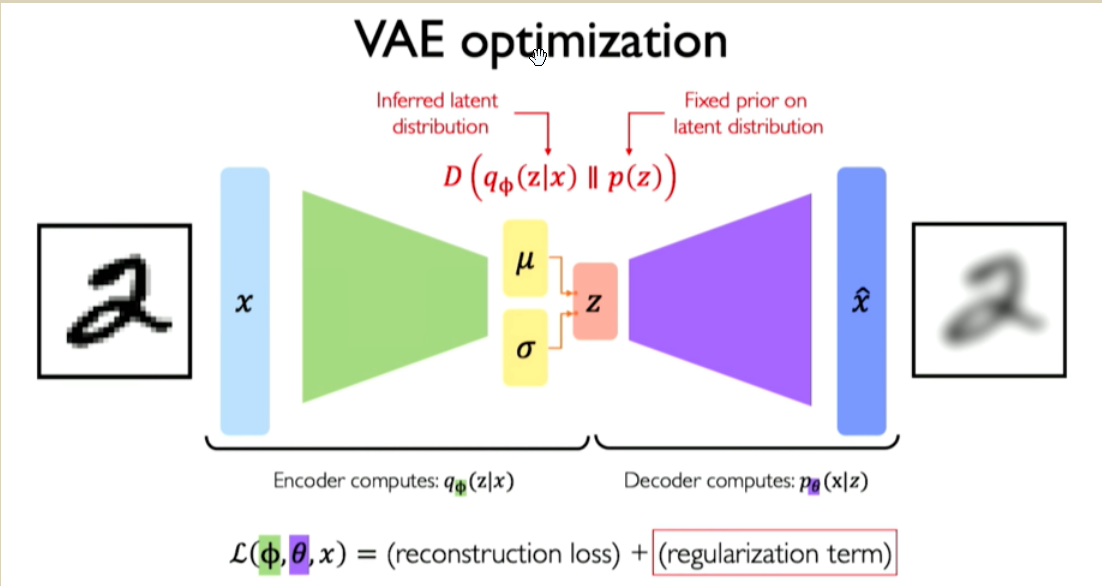
\includegraphics[width=0.7\textwidth]{images/vae.png}
\end{figure}

\begin{equation}
    D(q_\theta(z|x)||p(z))
\end{equation}

\textbf{Elementi:}
\begin{itemize}
    \item Inferred Latent Distribution: Distribuzione che hanno i dati di input
    \item Fixed Prior Latent Distribution: Distribuzione che vogliamo avere nel latent
          space
\end{itemize}

\textbf{Ad esempio}, nei normali Autoencoder, abbiamo che la distribuzione di input e la distribuzione di $z$ che viene fuori
non hanno niente a che fare. Cioè, non sappiamo niente a riguardo e non ci interessa.
Nei VAE, invece, vogliamo che la distribuzione di $z$ sia \textbf{normale}, perché con la distribuzione normale
si lavora in modo più stabile.

\begin{enumerate}
    \item Input X
    \item Decodifica X
    \item Si hanno due vettori di medie e varianze
    \item Si fa sampling e si ottiene $z$
    \item Si decodifica z
    \item Si ottiene il sample generato X'
\end{enumerate}

L'output di questa architettura prende il nome di \textbf{generated sample}.

Parlare di differenza tra regolarized e non regolarized dopo (inizio notebook)

\subsection{Regularization term e Reparametrization trick}

Il \textbf{Regularization Term} serve per fare in modo che la rete apprenda la
distribuzione nel \textbf{latent space}. Questo permtte di forzare di avere
$\mu = 0 \land \sigma = 1$

Il regularization term si chiama KL-Divergence e si calcola come segue:
\begin{equation}
    \frac{1}{2}\sum_{j=0}^{k-1}(\sigma_j+\mu^2_j - 1 - log(\sigma_j))
\end{equation}

\begin{figure}
    \centering
    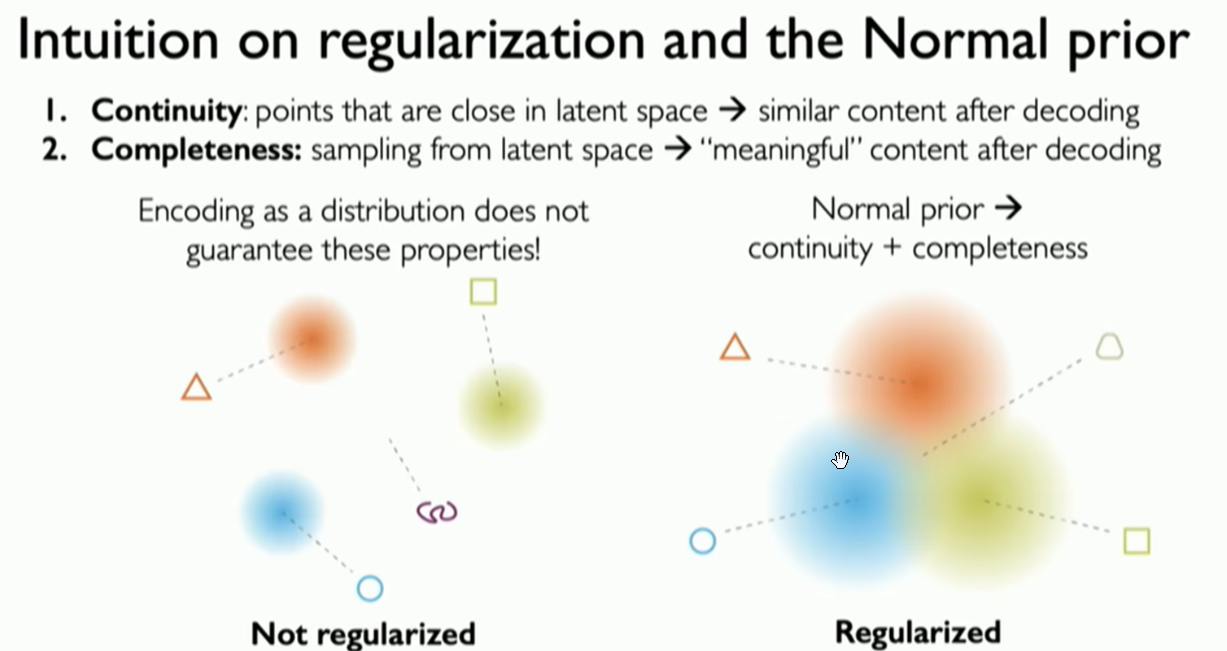
\includegraphics[width=0.7\textwidth]{images/vae2.png}
    \caption{Esempio di VAE}
\end{figure}

\begin{domanda}(Qual è la condizione per trainare una NN?)
\end{domanda}

Che la funzione sia \textbf{differenziabile}. Ma abbiamo un problema. Se dal
tra \textbf{mean e standard deviation} facciamo sampling, otteniamo una
distribuzione. Questo \textbf{non è differenziabile}. E qui entra in gioco il
\textbf{reparametrization trick}. Il trick è quello di \textbf{wrappare} questo
processo in una funzione che sia differenziabile.

\begin{figure}[H]
    \centering
    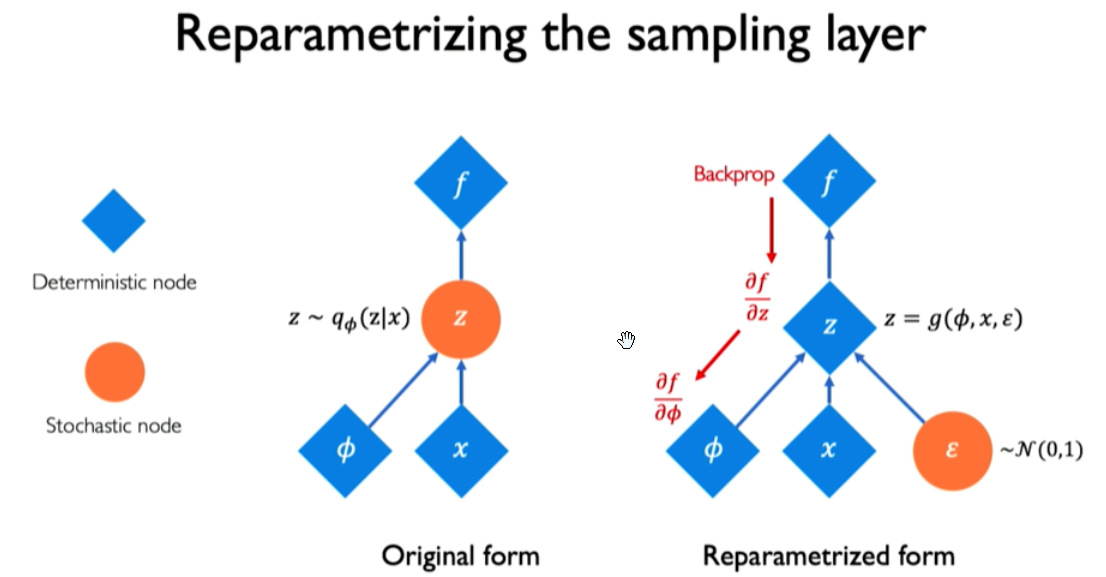
\includegraphics[width=0.7\textwidth]{images/reparametrization.png}
    \caption{Reparametrization trick}
\end{figure}

Oltre all'input, si aggiunge un elemento $\varepsilon$ che è un sample da una
distribuzione normale, lo consideriamo come \textbf{noise}. Questo noise è
\textbf{non deterministico} ed è differenziabile.

In questo modo, la funzione è differenziabile e si può fare backpropagation,
andando a cambiare i pesi dell'\textbf{encoder} e del \textbf{decoder}.

Senza di questo non potremmo farlo perché $z$ è un \textbf{random process} e
non è differenziabile.

\begin{lstlisting}[language=Python, caption={Esempio di VAE}]
from tensorflow import keras 

class Sampling(keras.layers.Layer):
    """Uses (z_mean, z_log_var) to sample z, the vector encoding a digit."""

    def call(self, inputs):
        z_mean, z_log_var = inputs
        batch = tf.shape(z_mean)[0]
        dim = tf.shape(z_mean)[1]
        epsilon = tf.keras.backend.random_normal(shape=(batch, dim))
        return z_mean + tf.exp(0.5 * z_log_var) * epsilon

from tensorflow.keras.datasets import fashion_mnist
import numpy as np

(x_train, _), (x_test, _) = fashion_mnist.load_data()
mnist_fashion = np.concatenate([x_train, x_test], axis=0)
mnist_fashion = np.expand_dims(mnist_fashion, -1).astype("float32") / 255

mnist_fashion.shape
\end{lstlisting}

\begin{lstlisting}[language=Python, caption={Esempio di VAE}]
    
latent_dim = 50
#50 medie e 50 deviazioni standard

encoder_inputs = keras.Input(shape=(28, 28, 1))
x = layers.Conv2D(32, 3, activation="relu", strides=2, padding="same")(encoder_inputs)
x = layers.Conv2D(64, 3, activation="relu", strides=2, padding="same")(x)
x = layers.Flatten()(x)
x = layers.Dense(100, activation="relu")(x)
z_mean = layers.Dense(latent_dim, name="z_mean")(x)
z_log_var = layers.Dense(latent_dim, name="z_log_var")(x)
z = Sampling()([z_mean, z_log_var])
encoder = keras.Model(encoder_inputs, [z_mean, z_log_var, z], name="encoder")
encoder.summary()
\end{lstlisting}

\begin{lstlisting}[language=Python, caption={Esempio di VAE}]
latent_inputs = keras.Input(shape=(latent_dim,))
x = layers.Dense(7 * 7 * 64, activation="relu")(latent_inputs)
x = layers.Reshape((7, 7, 64))(x)
x = layers.Conv2DTranspose(64, 3, activation="relu", strides=2, padding="same")(x)
x = layers.Conv2DTranspose(32, 3, activation="relu", strides=2, padding="same")(x)
decoder_outputs = layers.Conv2DTranspose(1, 3, activation="sigmoid", padding="same")(x)
decoder = keras.Model(latent_inputs, decoder_outputs, name="decoder")
decoder.summary()
\end{lstlisting}

\begin{lstlisting}[language=Python, caption={Esempio di VAE}]
    
class VAE(keras.Model):

    def __init__(self, encoder, decoder, **kwargs):
        super(VAE,self).init(kwargs)

        self.encoder = encoder
        self.decoder = decoder
        self.totallosstracker = keras.metrics.Mean(name="totalloss")
        self.reconstructionlosstracker = keras.metrics.Mean(name="reconstructionloss")
        self.kllosstracker = keras.metrics.Mean(name="klloss")

    def trainstep(self, data):

        with tf.GradientTape() as tape:

            zmean, zlogvar, z = self.encoder(data)

            reconstruction = self.decoder(z)

            reconstructionloss = tf.reducemean(
                tf.reducesum(keras.losses.binarycrossentropy(data, reconstruction), axis=(1, 2)))

            klloss = -0.5 * (1 + zlogvar - tf.square(zmean) - tf.exp(zlogvar))
            klloss = tf.reducemean(tf.reducesum(klloss, axis=1))

            totalloss = reconstructionloss + klloss

        grads = tape.gradient(totalloss, self.trainableweights)
        self.optimizer.applygradients(zip(grads, self.trainableweights))
        self.totallosstracker.updatestate(totalloss)
        self.reconstructionlosstracker.updatestate(reconstructionloss)
        self.kllosstracker.updatestate(klloss)

        return {
            "loss": self.totallosstracker.result(),
            "reconstructionloss": self.reconstructionlosstracker.result(),
            "klloss": self.kllosstracker.result(),
        }
\end{lstlisting}

\section{Recurrent Neural Network e Natural Language Processing (RNN e NLP)}
\subsection{RNN e LSTM}
Stiamo pensando in uno spazio a tre dimensioni:
\[
    Input, Output, Time
\]

Nelle RNN ogni neurone prende in input l'output del neurone precedente.
\begin{figure}[H]
    \centering
    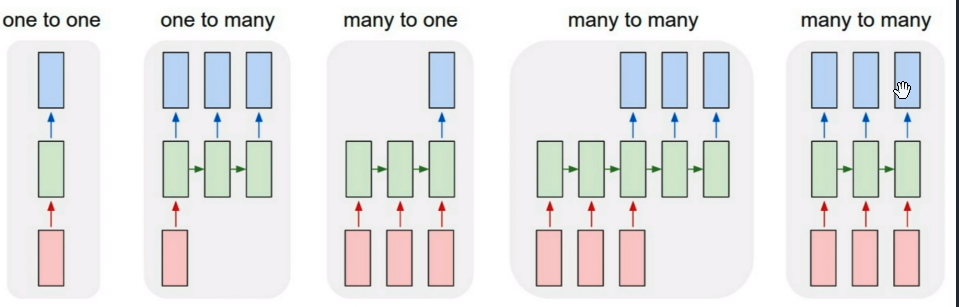
\includegraphics[width=0.7\textwidth]{images/archRNN.png}
    \caption{RNN}
\end{figure}

\begin{itemize}
    \item One-to-one - architettura classica di rete neurale feed-forward, con un input e
          ci aspettiamo un output.
    \item One-to-many - ad es. didascalia dell'immagine. Abbiamo un'immagine come input
          di dimensione fissa e l'output può essere parole o frasi che variano in
          lunghezza.
    \item Many-to-one ad es. classificazione del sentimento. Ci si aspetta che l'input
          sia una sequenza di parole o addirittura paragrafi di parole. L'output può
          essere un output di regressione con valori continui che rappresentano la
          probabilità di avere un sentimento positivo.
    \item Many-to-many - traduzione automatica come in Google translate. L'input potrebbe
          essere una frase inglese di lunghezza variabile e l'output sarà la stessa frase
          in una lingua diversa che ha anche una lunghezza variabile.
\end{itemize}

L'ultimo modello many-to-many può essere utilizzato per la classificazione
video a livello di frame. Inserisci ogni frame di un video nella rete neurale e
aspettati un output immediato. Tuttavia, poiché i frame sono generalmente
dipendenti l'uno dall'altro, è necessario che la rete propaghi il suo stato
nascosto dal precedente al successivo. Quindi, abbiamo bisogno di una rete
neurale ricorrente per questo tipo di attività. Si utilizza un'architettura
particolare per le RNN, chiamata \textbf{Long Short Term Memory (LSTM)}.
\begin{figure}[H]
    \centering
    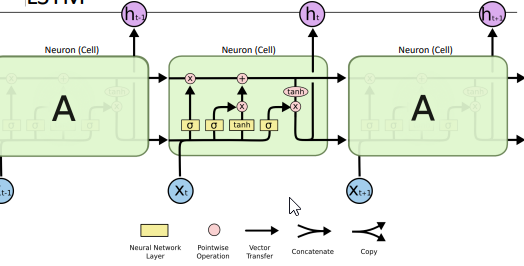
\includegraphics[width=0.7\textwidth]{images/LSTM.png}
    \caption{LSTM}
\end{figure}

\textbf{Forget Gate} - decide quali informazioni dalla memoria a lungo termine devono
essere mantenute o scartate e ciò viene fatto moltiplicando la memoria a lungo
termine in arrivo (freccia in arrivo superiore) per un vettore di dimenticanza
generato dall'input corrente e dalla memoria a breve termine in arrivo (freccia
inferiore).

\textbf{Input Gate} - decide quali informazioni verranno memorizzate nella memoria a
lungo termine. Funziona solo con le informazioni dall'input corrente e dalla
memoria a breve termine del passaggio precedente. A questo cancello, filtra le
informazioni dalle variabili che non sono utili.

\textbf{Output Gate} - prende l'input corrente, la memoria a breve termine precedente e
la memoria a lungo termine appena calcolata per produrre una nuova memoria a
breve termine che verrà passata alla cella nel passaggio di tempo successivo.
L'output del passaggio di tempo corrente può anche essere estratto da questo
stato nascosto. 

Praticamente, dai miei appunti successivi, ho capito che il \textbf{layer di sopra} è ciò che
tiene lo stato della cella, che sia precedente, corrente e successivo. Successivamente, oltre a questo, 
i vari layer aiutano la singola cella a capire quali informazioni salvare e quali non salvare. Inoltre, bisogna 
anche capire cosa mandare al prossimo layer, quindi per forza ci vuole una regolarizzazione 
che aiuti questo processo.

In linea di massima, questo è il funzionamento delle \textbf{LSTM}.


\subsection{NLP}

Le reti neurali lavorano con \textbf{numeri}. Nel natural language processing
si lavora con dei \textbf{testi} che sono delle \textbf{sequenze} di parole.

\textbf{Proposta 1: One Hot Encoding}:
Si potrebbe pensare ad un \textbf{one hot encoding}, ma questo sarebbe troppo
costoso, perché se dovessimo pensare ad un OHE di un vocabolario di 1000 parole,
questo crescerebbe in modo esponenziale

\textbf{Proposta 2:Ogni parola un unico numero}:
Problema da prendere dal notebook

\textbf{Proposta finale: Word Embedding}: Questa proposta è vincente perché permette di avere
una rappresentazione delle parole mantenendo un'importante proprietà: la \textbf{somiglianza} tra esse. Praticamente
un embedding è un vettore di valori in floating point. Invece di hard-codare i valori del vettore, si
trattano come valori da \textbf{allenare}.

%tabella per "cat on mat " a 4 dimensioni 
\begin{table}[H]
    \centering
    \begin{tabular}{|c|c|c|c|}
        \hline
        cat & 0.2 & 0.1 & \\
        \hline
        on  & 0.1 & 0.9 & \\
        \hline
        mat & 0.1 & 0.9 & \\
        \hline
    \end{tabular}
    \caption{Esempio di Word Embedding}
\end{table}

\subsection{Come si lavora con i Word Embedding?}

\subsubsection{Encoder}
\begin{lstlisting}[language=Python, caption={Esempio di Word Embedding}]
VOCAB_SIZE = 1000
#Per usare testo si usa un layer TextVectorization
encoder = tf.keras.layers.TextVectorization(max_tokens=VOCAB_SIZE)
encoder.adapt(train_dataset.map(lambda text, label: text))

#Parole piu usate nel dataset
vocab = np.array(encoder.get_vocabulary())
vocab[:20]

#Come sono encodate le parole
encoded_example = encoder(example)[:3].numpy()
encoded_example

#Ad esempio, l'encoding viene fatto stampando l'indice della parola nel vocabolario


\end{lstlisting}

\textbf{Nota:} Limitando il vocabolario non permette sempre di fare reverse tra indice e parola, perché la parola all'interno della frase potrebbe non essere all'interno delle top parole usate all'interno del nostro vocabolario.

\newpage